\documentclass[]{article}

% Imported Packages
%------------------------------------------------------------------------------
\usepackage{amssymb}
\usepackage{amstext}
\usepackage{amsthm}
\usepackage{amsmath}
\usepackage{enumerate}
\usepackage{fancyhdr}
\usepackage[margin=1in]{geometry}
\usepackage{graphicx}
%\usepackage{extarrows}
%\usepackage{setspace}
%\usepackage{xcolor}
\usepackage{color}
\usepackage{parskip}
%------------------------------------------------------------------------------

% Header and Footer
%------------------------------------------------------------------------------
\pagestyle{plain}  
\renewcommand\headrulewidth{0.4pt}                                      
\renewcommand\footrulewidth{0.4pt}                                    
%------------------------------------------------------------------------------

% Title Details
%------------------------------------------------------------------------------
\title{Deliverable \#1 Template : Software Requirement Specification (\textbf{SRS})}
\author{SE 3A04: Software Design II -- Large System Design}
\date{}
                            
%------------------------------------------------------------------------------

% Document
%------------------------------------------------------------------------------
\begin{document}

\maketitle\begin{center}
\noindent{\bf Tutorial Number:} T03\\
{\bf Group Number:} G8 \\
{\bf Group Members:} 
\begin{itemize} \centering
	\item Adam Mak
	\item Eric Chen
	\item Justin Ho
	\item Ahmad Hamadi
	\item Kevin Ishak
	\item Jonathan Jiang
\end{itemize}
\end{center}

\newpage
\section{Introduction}
\label{sec:introduction}
% Begin Section

\subsection{Purpose}
\label{sub:purpose}
% Begin SubSection
The purpose of this \textbf{SRS} is to define the functionality and characteristics that the carpool app should have. It should provide a detailed overview of all the processes and systems that needs to be present in the final product. The \textbf{SRS} will have a descriptive model, which will be represented visually in the form of a use-case diagram.
\begin{itemize}
	\item Developers
	\item UI/UX Designers
	\item Product Managers
	\item Engineers
	\item System Architects
	\item Quality Assurance Testers
\end{itemize}
% End SubSection

\subsection{Scope}
\label{sub:scope}
% Begin SubSection
The software product is a taxi carpool service. It will provide a communication environment for passengers to carpool via taxis. This service is not meant to be replacement for taxi services (i.e. Uber-like services).

The objective of the software (local taxi system) being implemented is to transport users from one destination to another using a carpool method. This software allows user to enter a destination along with some optional search criteria that they want to arrive at. The software will then match the user with a taxi nearby which may or may not carry other individuals who are travelling in the same general direction. This benefits both the users, taxi driver as well as the environment by as it helps reduce costs, whether it be the fare for the ride or the reduction in environmental pollutants by the means of carpooling.

There are no higher-level specifications that exist, thus, any lower-level specifications must be consistent with this document, as it is the highest-level specification.
% End SubSection

\subsection{Definitions, Acronyms, and Abbreviations}
\label{sub:definitions_acronyms_and_abbreviations}
% Begin SubSection
\begin{center} \begin{tabular} {|c|p{35em}|}
	\hline
	\textbf{Abbreviation/Acronym} & \textbf{Definition} \\
	\hline \hline
	API & Application Programming Interface \\
	\hline
	Carpool & To collectively share a ride (either to help reduce the cost of transit or as an act of being more environmentally “green”) \\
	\hline
	DBMS & Database Management System \\
	\hline
	GoPlay Store & The default Android distribution platform \\
	\hline
	SMS & Software Requirements Specification \\
	\hline
	SRS & Simple Message Service \\
	\hline
	Passengers & A terminology for both the carpoolers and the requesters\\
	\hline
\end{tabular} \end{center}
% End SubSection

\subsection{References}
\label{sub:references}
% Begin SubSection
APA references sorted by occurence of when they appear in this document.
\begin{enumerate}
	\item Simic, S. (2022, December 13). 7 ways to reduce server response time {Improve your server speed}. Knowledge Base by phoenixNAP. Retrieved March 5, 2023, from https://phoenixnap.com/kb/reduce-server-response-time\#:~:text=Google\%20recommends\%20you\%20aim\%20for,on\%20the\%20users'\%20geographical\%20positions.
	\item Earls, A. R. (2019, July 19). Best practices for negotiating a SAAS SLA: TechTarget. Cloud Computing. Retrieved March 5, 2023, from https://www.techtarget.com/searchcloudcomputing/tip/Negotiate-a-SaaS-SLA-for-compliance-uptime-considerations
	\item What is an audit? everything about the 3 types of audits. Ageras. (n.d.). Retrieved March 5, 2023, from https://www.ageras.com/blog/what-is-an-audit
	\item Office of the Privacy Commissioner of Canada. (2021, December 8). The Personal Information Protection and Electronic Documents Act (PIPEDA). Office of the Privacy Commissioner of Canada. Retrieved March 5, 2023, from https://www.priv.gc.ca/en/privacy-topics/privacy-laws-in-canada/the-personal-information-protection-and-electronic-documents-act-pipeda/
	\item Home. TTA. (1970, February 7). Retrieved March 5, 2023, from https://www.thetransportationalliance.org/
	\item Business insurance. NFP. (n.d.). Retrieved March 5, 2023, from https://www.nfp.ca/business-insurance/industry-expertise/taxis-limousines-and-busses
	\item Taxi fare. Taxi Fare - TLC. (n.d.). Retrieved March 5, 2023, from https://www.nyc.gov/site/tlc/passengers/taxi-fare.page
\end{enumerate}
% End SubSection

\subsection{Overview}
\label{sub:overview}
% Begin SubSection
In the order of occurrence, the remainder of the \textbf{SRS} contains an overview of the system, which includes product perspective, product functions, user characteristics, constraints, and dependencies. The \textbf{SRS} will have a descriptive model, which will be represented visually in the form of a use-case diagram. Furthermore, the document also includes various system-specific requirements which are consist of functional and non-functional requirements.  Finally, at the end of the document, there is a record which represents the division of labour of all contributors to the project.
% End SubSection

% End Section

\section{Overall Product Description}
\label{sec:overall_description}
% Begin Section

\subsection{Product Perspective}
\label{sub:product_perspective}
% Begin SubSection
The carpool app product is independent and self-contained, as it does not build upon any existing products/applications. However, the standalone system uses and owns interfaces to and from external systems, such as hardware, users, databases, and other \textbf{API}'s, to provide essential functionality to the app. Figure \ref{fig:blockdiagram} shows how these external systems will interact in a block diagram.

The carpooling app is developed for Android devices, providing users owning these devices with easy access to this service. Also, the app's user interface interacts with an Android device to allow users to see information and interact with the application through a touchscreen.

The app sends and receives data from a database that stores information about users, rides, route information, and other related data. This is managed by a \textbf{DBMS}.

The carpooling app uses the Google Map \textbf{API} to provide maps and location-related services such as route planning and estimating travel times. The \textbf{API} provides information about the locations of users and destinations, as well as real-time traffic data, to help drivers make more informed decisions about their routes.

To protect sensitive information such as passwords, payment information, transmitted messages, and other confidential data, the carpooling app uses a cryptosystem to encrypt this information before it is stored in the \textbf{DBMS}. When the data is needed, it is decrypted and used by the app. This ensures that information is protected from unauthorized access.

The carpooling app uses \textbf{SMS} functionality to provide communication between users to provide updates, confirm ride details, and more. For instance, when a ride is requested, the app may send a message to the driver to notify them of the request, and then another message to the passenger to confirm the ride details.

\begin{figure}[h!]
	\centering
	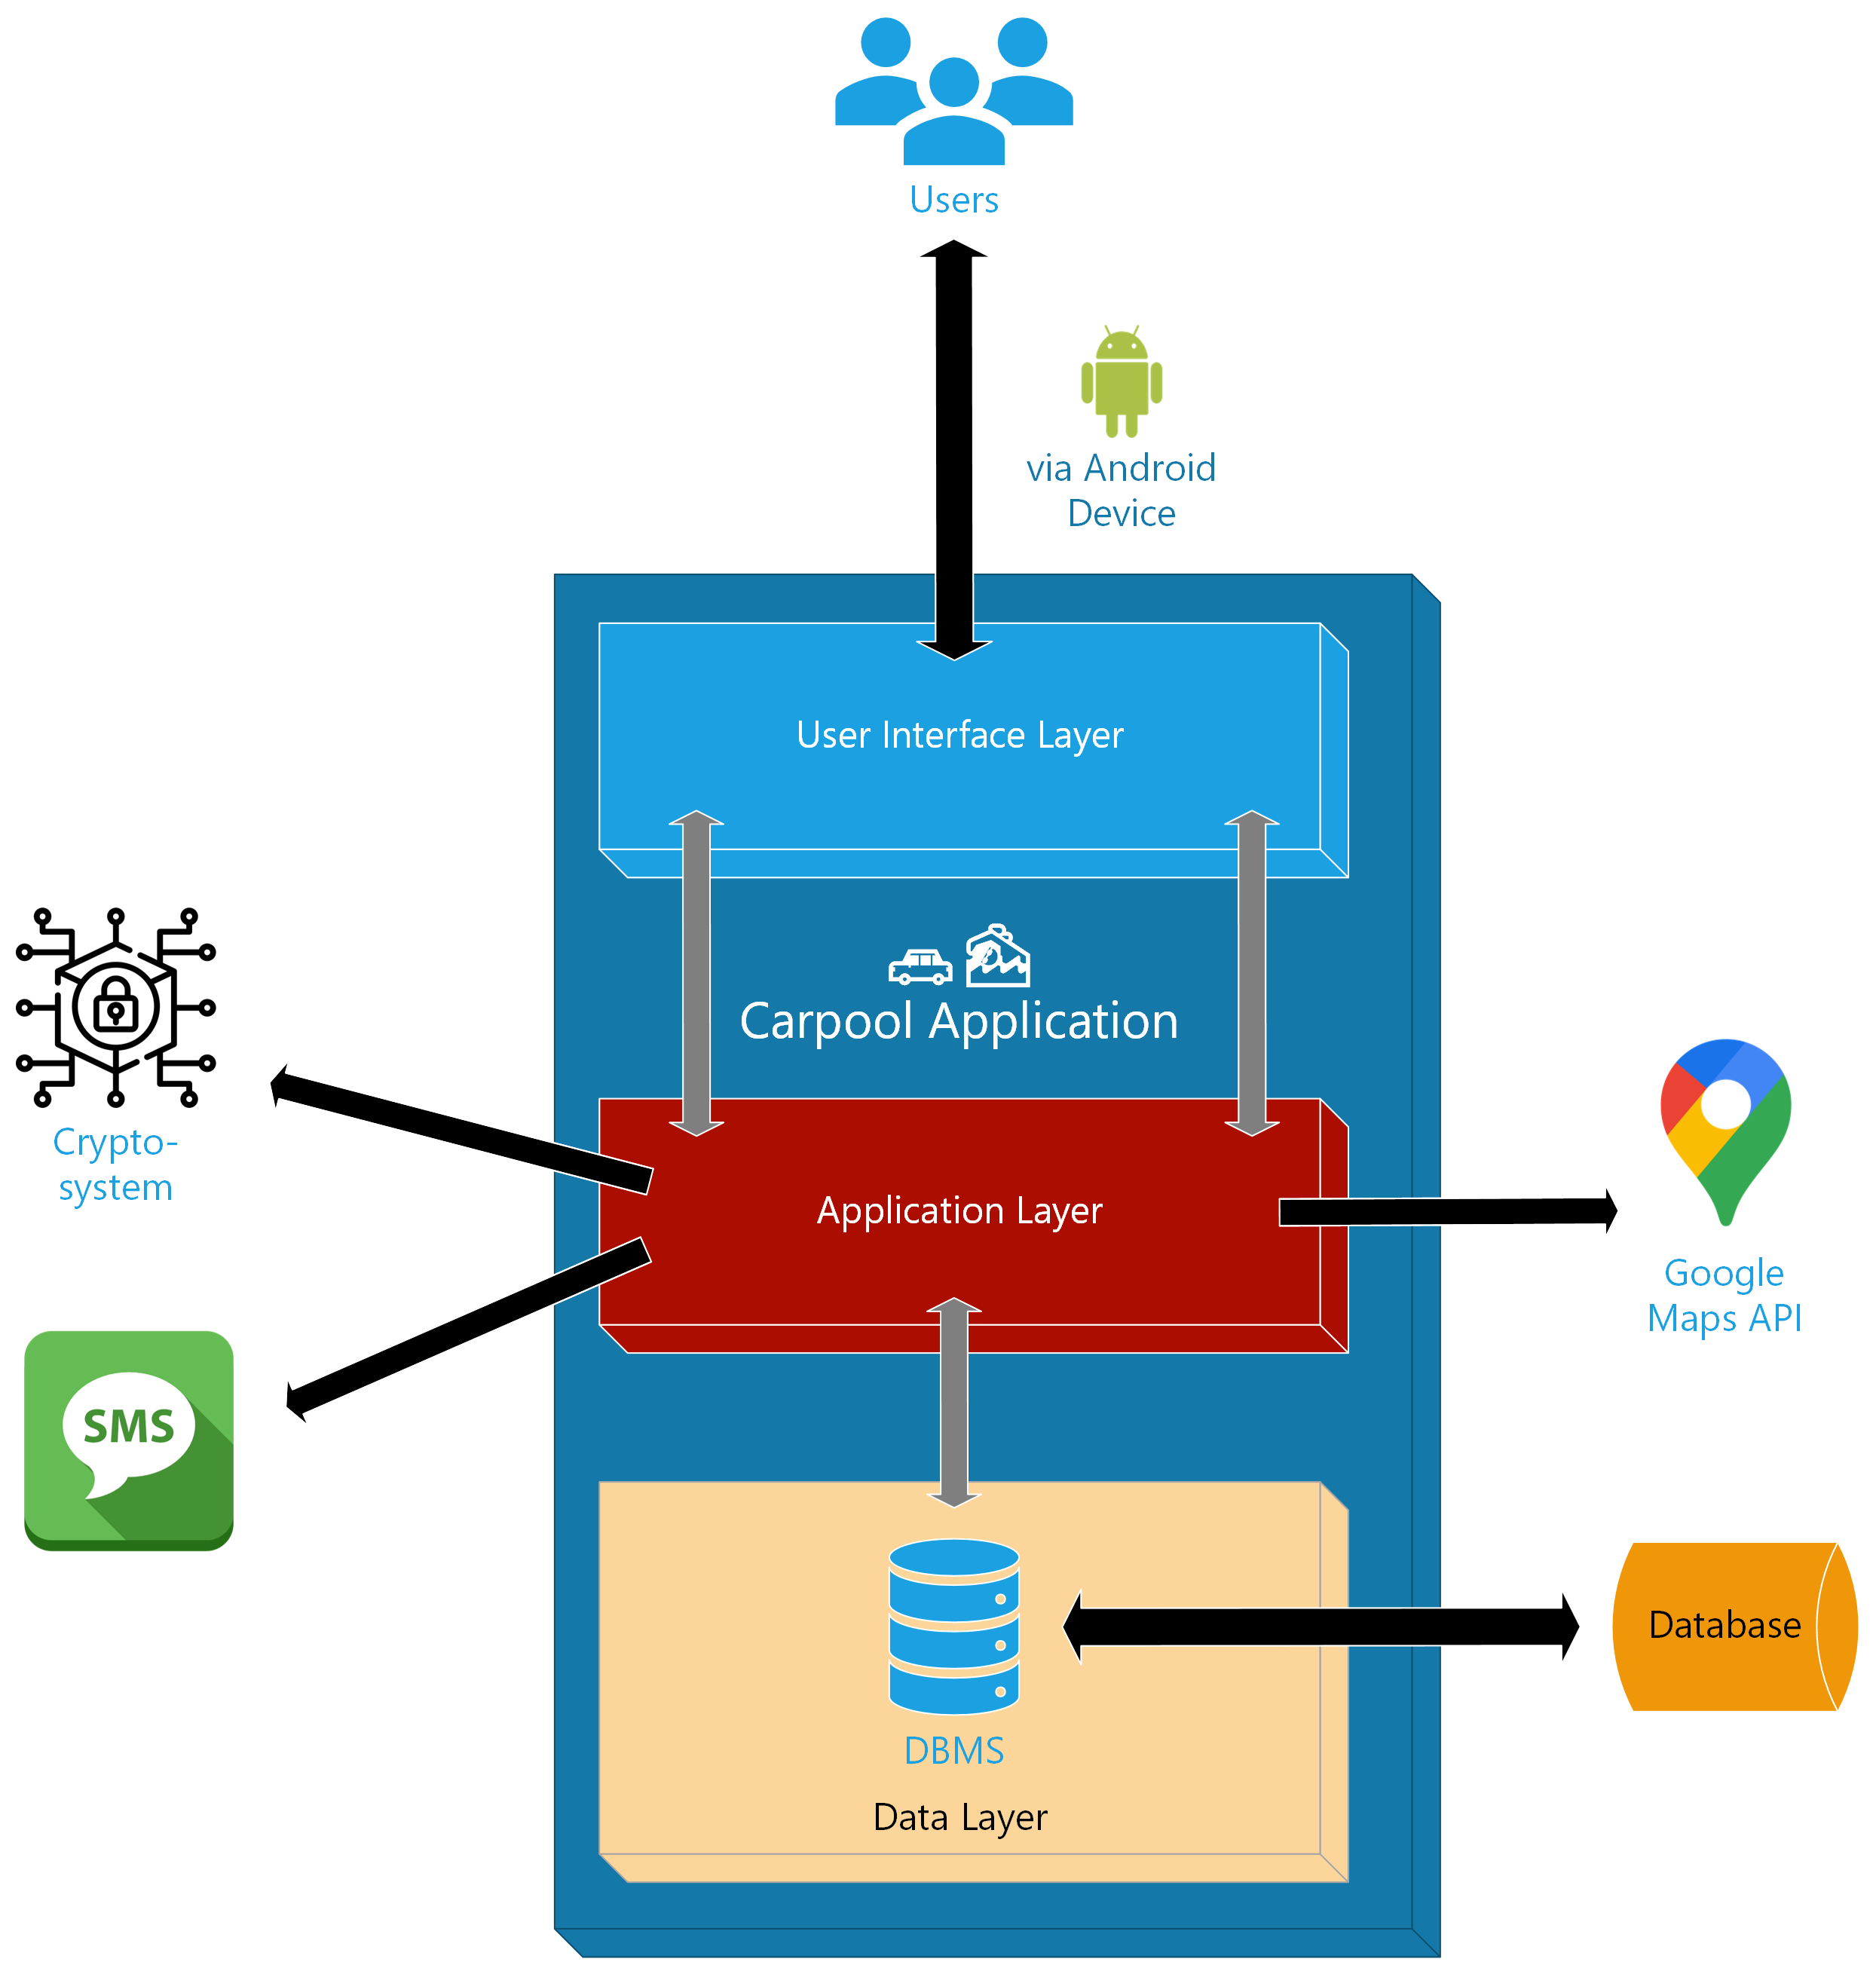
\includegraphics[width=30em]{ProductPerspectiveBlockDiagram.png}
	\caption{A block diagram showing the major layers of the carpooling application, interconnections, and external interfaces.}
	\label{fig:blockdiagram}
\end{figure}
% End SubSection

\subsection{Product Functions}
\label{sub:product_functions}
% Begin SubSection
\begin{itemize}
	\item App should compare carpool price with non carpool price and display the money saved as a point system.
	\item App should allow carpoolers to setup/join other carpoolers using the app.
	\item When requesting a carpool, carpoolers should be able to filter through different travel options (i.e. sort by closest cab/highest rated cab driver). The app should return a list of cab options according to the specification.
	\item Carpoolers looking to set up a carpool should be able to input the taxi ID , destination, maximum number of other carpoolers, as well as potential auxiliary information. They system should post this info and allow other carpoolers to join.
	\item Users should be able to create and delete accounts, which the system should store.
	\item The system should check if a user that wants to request/setup a carpool is a registered user. It should reject unregistered users.
	\item App should have a reward system that allows users to obtain free rides based on their accumulated cost savings.
	\item App should have a points system that keeps track of costs saved, and reward free rides once a carpooler exceeds a certain number of points.
\end{itemize}
% End SubSection

\subsection{User Characteristics}
\label{sub:user_characteristics}
% Begin SubSection
Users include both passengers and drivers, of which education level may vary. The users of the product are expected to have a basic knowledge of technology and are familiar with smartphones, which the app is developed for. Also, users must 16 years of age or older to use the app.
% End SubSection

\subsection{Constraints}
\label{sub:constraints}
% Begin SubSection
\begin{itemize}
	\item Legal and regulatory restrictions: The developer needs to ensure that the application complies with the local laws and regulations.
	\item Technical limitations: The developer may face limitations with regards to the technology used to build the application, such as compatibility with different platforms, scalability, and security.
	\item Budget and resources: The availability of financial and human resources can impact the scope and timeline of the project.
	\item Time limits: The project must be completed within the span of 4 months.
\end{itemize}
% End SubSection

\subsection{Assumptions and Dependencies}
\label{sub:assumptions_and_dependencies}
% Begin SubSection
The carpool app will be available for installation/download through the Apple and Google Play store for users to use. It is assumed that Apple/Google Play will streamline our app upon the necessary guidelines being met (I.e., Safety, Privacy, Performance, Business, Design, Legal).

It is assumed that the Google Maps \textbf{API} will be available to use with an 100\% uptime which our carpool app will utilize to plan its routes and navigate users around cities. If the Google Maps \textbf{API}, for some extenuating circumstances, is unable to provide the services for route navigation, then another GIS \textbf{API} system may have to be utilized (e.g., OpenLayers, ESRI, etc…).

A primary telecommunication company will be managing the \textbf{SMS} traffic of the carpool app as the app makes use of \textbf{SMS} functionality to inform users about the status of their ride. If for some reason, any of the telecommunication companies listed within this \textbf{SRS} document disbands, terminates the contract or breach some sort of confidentiality between both parties, and/or something similar in nature, then the \textbf{SRS} might have to change accordingly to fill up the vacant \textbf{SMS} management company.

It is assumed that the carpool app will be systematically be calculating the cost of the trip per person on a reduced per mileage basis. 
% End SubSection

\subsection{Apportioning of Requirements}
\label{sub:apportioning_of_requirements}
% Begin SubSection
The following requirements are usually delayed until later versions to meet the initial launch deadline and budget, or to focus on delivering the most valuable features to users first.

\begin{enumerate}
	\item Advanced features: These are features that are not essential to the core functionality of the app, but can be added later as the app evolves.
	\begin{itemize}
		\item[-] For example, an in-app tipping feature, or integration with a rewards program. 
	\end{itemize}
	\item Non-critical performance optimizations: Improving the app's performance can be a continuous process, and some optimizations can be deferred until later versions.
	\begin{itemize}
		\item[-] For example, optimizations that improve the app's speed, reliability or efficiency, but are not essential to its basic functionality.  
	\end{itemize}
	\item Complex user interfaces: Advanced user interfaces can be time-consuming to develop and may be deferred in favor of a simpler interface in the initial release. 
	\begin{itemize}
		\item[-] For example, a more sophisticated design that includes augmented reality, or a chatbot interface.  
	\end{itemize}
	\item Integrations with third-party systems: Integrating the app with other systems can be a significant effort, and this work may be deferred until later versions. 
	\begin{itemize}
		\item[-] For example, integration with a payment system, or with a local transit system. 
	\end{itemize}
	\item Support for older platforms: Supporting older platforms can be time-consuming, and this work may be deferred until later versions or only supported for critical security and bug fixes.
	\begin{itemize}
		\item[-] For example, supporting older versions of the iOS or Android operating systems. 
	\end{itemize}
\end{enumerate}

\noindent It is important to prioritize the most critical requirements, such as the core functionality of booking a ride, and ensuring that the app is easy to use. Other requirements can be deferred until future versions to meet the initial launch deadline and budget. 
% End SubSection

% End Section
\newpage\section{Use Case Diagram}
\label{sec:use_case_diagram}
% Begin Section
\begin{figure}[h]
	\centering
	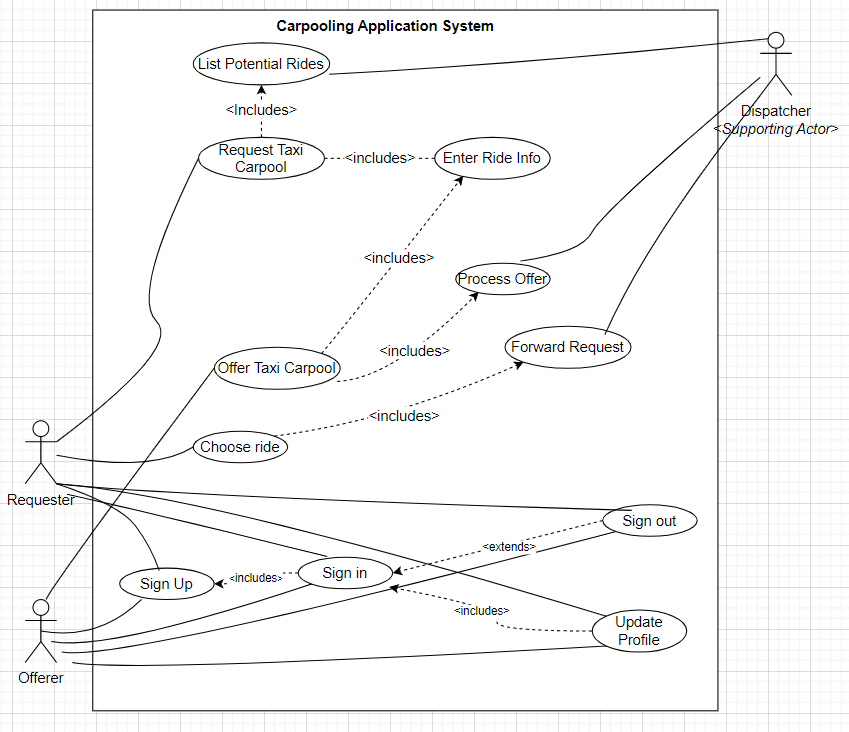
\includegraphics[width=30em]{usecase_v3.png}
	\caption{Use case diagram of the carpooling application.}
	\label{fig:usecase}
\end{figure}
%% End Section

\section{Highlights of Functional Requirements}
\label{sec:functional_requirements}
% Begin Section
The business events we will present are:
\begin{enumerate}
    \item[] \textbf{BE1.} Request a ride
    \item[] \textbf{BE2.} Arrive at destination
    \item[] \textbf{BE3.} Setup/Update user profile/account information
    \item[] \textbf{BE4.} Offer a ride
    \item[] \textbf{BE5.} Login/Logout of an account
    \item[] \textbf{BE6.} Redeem a free ride
    \item[] \textbf{BE7.} Delete user profile
\end{enumerate}

The viewpoints we will consider are:
\begin{enumerate}
    \item[] \textbf{VP1.} Requester
    \item[] \textbf{VP2.} Offerer
\end{enumerate}

\noindent {\bf Interpretation:} Specify any liberties you took in interpreting business events, if necessary.\\

\begin{enumerate}[{\bf BE1.}]
	\item Partake in a ride
		\begin{enumerate}[{\bf VP1.}]
			\item Requesters \\
			\noindent\fbox{
				\parbox{0.85\textwidth}{
					\begin{itemize}
						\item {$S_{1}$:} System asks requester for a pickup location and a destination point and allows them to input a search preference (nearest cab, highest rating first, find specific offerer).
						\item {$E_{1}$:} Passenger inputs a pickup location and a destination point, as well as any optional information.
						\item {$S_{2}$:} System checks if there are any available carpoolers. \begin{itemize}
							\item[] $S_{2.1}$: There are no available carpool events. The system displays that there are no available carpools \textbf{\color{red}\textlangle Branch EXIT \textrangle}.
							\item[]$S_{2.2}$: There are available carpool events. The system lists out the Carpool events that correspond to the users inputted preferences, as well as a choice to reject all carpool events.
						\end{itemize}
						\item {$E_{2}$:} User decides whether to choose any of the carpool events. \begin{itemize}
							\item[] $E_{2.1}$: Requester rejects all carpool events. \textbf{\color{red}\textlangle Branch EXIT \textrangle}
							\item[]$E_{2.2}$: Requester chooses a carpool event.
						\end{itemize}
						\item {$S_{3}$:} System notifies offerer of the request.
					\end{itemize}
				}
			}
			\item Offerer \\
				\noindent\fbox{\parbox{0.85\textwidth}{N/A}}
		\end{enumerate}
		{\bf Global Scenario:}\\
		\noindent\fbox{
			\parbox{0.85\textwidth}{
				\begin{itemize}
					\item {$S_{1}$:} System asks requester for a pickup location and a destination point and allows them to input a search preference (nearest cab, highest rating first, find specific offerer).
					\item {$E_{1}$:} Passenger inputs a pickup location and a destination point, as well as any optional information.
					\item {$S_{2}$:} System checks if there are any available carpoolers. \begin{itemize}
						\item[] $S_{2.1}$: There are no available carpool events. The system displays that there are no available carpools \textbf{\color{red}\textlangle Branch EXIT \textrangle}.
						\item[]$S_{2.2}$: There are available carpool events. The system lists out the Carpool events that correspond to the users inputted preferences, as well as a choice to reject all carpool events.
					\end{itemize}
					\item {$E_{2}$:} User decides whether to choose any of the carpool events. \begin{itemize}
						\item[] $E_{2.1}$: Requester rejects all carpool events. \textbf{\color{red}\textlangle Branch EXIT \textrangle}
						\item[]$E_{2.2}$: Requester chooses a carpool event.
					\end{itemize}
					\item {$S_{3}$:} System notifies offerer of the request.
				\end{itemize}
			}
		}
	\item Leaving a rating on the app
	\begin{enumerate}[{\bf VP1.}]
		\item Passenger (Requester and Offerer) \\
		\noindent\fbox{
			\parbox{0.85\textwidth}{
				\begin{itemize}
					\item {$S_{1}$:} System attempts to authenticate that the passenger has arrived at their destination point. \begin{itemize}
						\item[] $S_{1.1}$: System fails to authenticate that the passenger has arrived at the destination point. \textbf{\color{red}\textlangle Branch EXIT \textrangle}
						\item[]$S_{1.2}$: System successfully authenticates the passenger and displays a list of applicable (previous carpool partners) passengers to leave a review/rating (/5) for.
					\end{itemize}
					\item {$E_{1}$:} Passenger responds to the system. \begin{itemize}
						\item[] $E_{1.1}$: Passenger skips the review process. \textbf{\color{red}\textlangle Branch BE2.VP1.S3 \textrangle}
						\item[]$E_{1.2}$: Passenger inputs a valid response (i.e., gives a rating and a potential message response) to the system
					\end{itemize}
					\item {$S_{2}$:} System receives a valid response and updates the individual's profile with the new rating.
					\item {$E_{2}$:} Passenger is notified of the change(s) made or the cancellation process.
					\item {$S_{3}$:} System updates the user's profile with points accumulated from the ride and notifies the user about their updated amount.
					\item {$E_{3}$:} Passenger is notified and presses "OK".
					\item {$S_{4}$:} System redirects user to the home page.
				\end{itemize}
			}
		}
	\end{enumerate}
	{\bf Global Scenario:}\\
	\noindent\fbox{
		\parbox{0.85\textwidth}{
			\begin{itemize}
				\item {$S_{1}$:} System attempts to authenticate that the passenger has arrived at their destination point. \begin{itemize}
					\item[] $S_{1.1}$: System fails to authenticate that the passenger has arrived at the destination point. \textbf{\color{red}\textlangle Branch EXIT \textrangle}
					\item[]$S_{1.2}$: System successfully authenticates the passenger and displays a list of applicable (previous carpool partners) passengers to leave a review/rating (/5) for.
				\end{itemize}
				\item {$E_{1}$:} Passenger responds to the system. \begin{itemize}
					\item[] $E_{1.1}$: Passenger skips the review process. \textbf{\color{red}\textlangle Branch GS2.S3 \textrangle}
					\item[]$E_{1.2}$: Passenger inputs a valid response (i.e., gives a rating and a potential message response) to the system
				\end{itemize}
				\item {$S_{2}$:} System receives a valid response and updates the individual's profile with the new rating.
				\item {$E_{2}$:} Passenger is notified of the change(s) made or the cancellation process.
				\item {$S_{3}$:} System updates the user's profile with points accumulated from the ride and notifies the user about their updated amount.
				\item {$E_{3}$:} Passenger is notified and presses "OK".
				\item {$S_{4}$:} System redirects user to the home page.
			\end{itemize}
		}
	}
	\item Setup/Update user profile/account information
	\begin{enumerate}[{\bf VP1.}]
		\item Passenger \\
		\noindent\fbox{
			\parbox{0.85\textwidth}{
				\begin{itemize}
					\item {$S_{1}$:} System prompts passenger for personal information (Full name, phone number, email).
					\item {$E_{1}$:} Passenger responds to the system. \begin{itemize}
						\item[] $E_{1.1}$: Passenger does not make any new changes to their profile or discards their 
						current changes. \textbf{\color{red}\textlangle Branch EXIT \textrangle}
						\item[]$E_{1.2}$: Passenger makes new changes to their profile. 
					\end{itemize}
					\item {$S_{2}$:} System updates the personal information of user and allows carpool services under the account and returns the user back to the settings page.
				\end{itemize}
			}
		}
	\end{enumerate}
	{\bf Global Scenario:}\\
	\noindent\fbox{
		\parbox{0.85\textwidth}{
			\begin{itemize}
				\item {$S_{1}$:} System prompts passenger for personal information (Full name, phone number, email).
				\item {$E_{1}$:} Passenger responds to the system. \begin{itemize}
					\item[] $E_{1.1}$: Passenger does not make any new changes to their profile or discards their 
					current changes. \textbf{\color{red}\textlangle Branch EXIT \textrangle}
					\item[]$E_{1.2}$: Passenger makes new changes to their profile. 
				\end{itemize}
				\item {$S_{2}$:} System updates the personal information of user and allows carpool services under the account and returns the user back to the settings page.
			\end{itemize}
		}
	}
	\item Cancel a ride
	\begin{enumerate}[{\bf VP1.}]
		\item Passenger \\
		\noindent\fbox{
			\parbox{0.85\textwidth}{
				\begin{itemize}
					\item {$S_{1}$:} System re-asks user if they want to cancel the ride.
					\item {$E_{1}$:} User indicates that they are sure they want to cancel the ride.
					\item {$S_{2}$:} System notifies the driver that the ride has been canceled.
				\end{itemize}
			}
		}
		\item Driver \\
		\noindent\fbox{\parbox{0.85\textwidth}{N/A}}
	\end{enumerate}
	{\bf Global Scenario:}\\
	\noindent\fbox{
		\parbox{0.85\textwidth}{
			\begin{itemize}
				\item {$S_{1}$:} System re-asks user if they want to cancel the ride.
				\item {$E_{1}$:} User indicates that they are sure they want to cancel the ride.
				\item {$S_{2}$:} System notifies the driver that the ride has been canceled.
			\end{itemize}
		}
	}
	\item Login/logout of an account
	\begin{enumerate}[{\bf VP1.}]
		\item Passenger \\
		\noindent\fbox{
			\parbox{0.85\textwidth}{
				\begin{itemize}
					\item {$S_{1}$:} System prompts passenger for login information (username and password).
					\item {$E_{1}$:} Passenger inputs their information.
					\item {$S_{2}$:} System checks if username and password matches any accounts information. \begin{itemize}
						\item[] $S_{2.1}$: Customers login info matches an account and they are granted access.
						\item[]$S_{2.2}$: Customers login does not match an account \textbf{\color{red}\textlangle Branch to VP1.S1 \textrangle}
					\end{itemize}
				\end{itemize}
			}
		}
		\item Driver \\
		\noindent\fbox{\parbox{0.85\textwidth}{N/A}}
	\end{enumerate}
	{\bf Global Scenario:}\\
	\noindent\fbox{
		\parbox{0.85\textwidth}{
			\begin{itemize}
				\item {$S_{1}$:} System re-asks user if they want to cancel the ride.
				\item {$E_{1}$:} User indicates that they are sure they want to cancel the ride.
				\item {$S_{2}$:} System notifies the driver that the ride has been canceled.
			\end{itemize}
		}
	}
	\item Edit payment information
	\begin{enumerate}[{\bf VP1.}]
		\item Passenger \\
		\noindent\fbox{
			\parbox{0.85\textwidth}{
				\begin{itemize}
					\item {$S_{1}$:} System authenticates user login and displays current payment method information (e.g., cards/email/PayPal).
					\item {$E_{1}$:} User selects payment method desired to modify.
					\item {$S_{2}$:} System allows for modification of payment method.
					\item {$E_{1}$:} User inputs new information.
					\item {$S_{2}$:} System saves edited information to the database.
				\end{itemize}
			}
		}
		\item Driver \\
		\noindent\fbox{\parbox{0.85\textwidth}{N/A}}
	\end{enumerate}
	{\bf Global Scenario:}\\
	\noindent\fbox{
		\parbox{0.85\textwidth}{
			\begin{itemize}
				\item {$S_{1}$:} System authenticates user login and displays current payment method information (e.g., cards/email/PayPal).
				\item {$E_{1}$:} User selects payment method desired to modify.
				\item {$S_{2}$:} System allows for modification of payment method.
				\item {$E_{1}$:} User inputs new information.
				\item {$S_{2}$:} System saves edited information to the database.
			\end{itemize}
		}
	}
	\item Redeem a free ride
	\begin{enumerate}[{\bf VP1.}]
		\item Passenger \\
		\noindent\fbox{
			\parbox{0.85\textwidth}{
				\begin{itemize}
					\item {$S_{1}$:} System checks if the user has a free ride available. \begin{itemize}
						\item[] $S_{1.1}$: System confirms that the user has a free ride available. System prompts user for a 
						response with a display message: “Do you want to redeem a free ride?” 
						\item[]$S_{1.2}$: System confirms that the user does not currently have a free ride available. \textbf{\color{red}\textlangle Branch EXIT \textrangle}
					\end{itemize}
					\item {$E_{1}$:} User responds to the system's prompt. \begin{itemize}
						\item[] $E_{1.1}$: User responds with “No” and decides not to redeem a free ride. \textbf{\color{red}\textlangle Branch EXIT \textrangle}
						\item[]$E_{1.2}$: User responds with “Yes” and would like to redeem a free ride.
					\end{itemize}
					\item {$S_{2}$:} System consumes the free ride coupon and removes the coupon (remove one if the user has more than one free-ride coupon) from the user's list of coupons/promotions available.
					\item {$E_{2}$:} User proceeds with confirming their travel route. \textbf{\color{red}\textlangle Branch to BE1 \textrangle}
				\end{itemize}
			}
		}
		\item Driver \\
		\noindent\fbox{\parbox{0.85\textwidth}{N/A}}
	\end{enumerate}
	{\bf Global Scenario:}\\
	\noindent\fbox{
		\parbox{0.85\textwidth}{
			\begin{itemize}
				\item {$S_{1}$:} .
			\end{itemize}
		}
	}
\end{enumerate}

%End Section

\section{Non-Functional Requirements}
\label{sec:non-functional_requirements}

% Begin Section
\subsection{Look and Feel Requirements}
\label{sub:look_and_feel_requirements}
% Begin SubSection
\subsubsection{Appearance Requirements}
\label{ssub:appearance_requirements}
% Begin SubSubSection
\begin{enumerate}[{LF-A}1. ]
	\item The app should conform to a standardized colour scheme which is to be used throughout the app. The choice of colour should be consistent all throughout the app and the must provide enough vibrance amongst each other so that in no shape of form gives off a “dull” image.\\
	{\bf Rationale:} Having a modern aesthetic and consistent color scheme help create a more engaging and enjoyable user experience while also reinforcing the brand and establishing a sense of professionalism. The vibrance also makes the app more accessible for those with visual impairments.
	\item The app should be organized by related content with little to no cluttering of text/images to provide for visually appealing and easy to read navigation. The cluttering of text/images should follow a basis of having at minimum 5 vw/vh between unrelated images/text bodies and 2.5 vw/vh for related ones.\\
	{\bf Rationale:} Organizing content and following a reasonable minimum spacing guideline help create a visually appealing and user-friendly experience that is easy to navigate and accessible to all users.
	\item The font family will remain consistent throughout the interface of the app. The size of the font will be increased amongst reasonable intervals and there shall be no difference in text size which varies ever so slightly.  There shall not be font size of something of the sort: 13.5, 13.7 and 13.9. Instead, a font size with more appropriate intervals will be an interval of 10, 12, 16 as it provides an easy way to distinguish the size of the text and remain consistent all throughout the app.\\
	{\bf Rationale:} Consistent font sizes make it easier for users to read and understand the text. If there are variations in font size, it can cause confusion and make it difficult for users to read and comprehend the content. 
\end{enumerate}
% End SubSubSection

\subsubsection{Style Requirements}
\label{ssub:style_requirements}
% Begin SubSubSection
\begin{enumerate}[{LF-S}1. ]
	\item The app shall have a monochromatic appearance, with appropriate font size and font type.\\
	{\bf Rationale:} See rationale for LF-A1.
\end{enumerate}
% End SubSubSection

% End SubSection

\subsection{Usability and Humanity Requirements}
\label{sub:usability_and_humanity_requirements}
% Begin SubSection

\subsubsection{Ease of Use Requirements}
\label{ssub:ease_of_use_requirements}
% Begin SubSubSection
\begin{enumerate}[{UH-EOU}1. ]
	\item The app should be relatively easy to learn for beginners and should require no more than 3 minutes of tutorial time to learn. A tutorial will be provided upon creating of a new account that helps navigate the user through the app if they so choose to.
	\item ll accessibility and navigation buttons should be intuitive and easy to find. Likewise, the content should be organized in a way so that finding related content is relatively easy and intuitive.
	\item The app should be accessible, and convenient for the general public to use. The app shall allow users to create an account through various forms of media (e.g. Gmail OAuth, \textbf{SMS} Login, Apple Login, etc...) so that users with only one source of media are not limited.\\
	{\bf Rationale:} The requirement for all accessibility and navigation buttons to be intuitive and easy to find ensures that users can easily navigate the app's interface and access the content they need. Organizing related content in an easy and intuitive way improves user experience and minimizes frustration when searching for information.
\end{enumerate}
% End SubSubSection

\subsubsection{Personalization and Internationalization Requirements}
\label{ssub:personalization_and_internationalization_requirements}
% Begin SubSubSection
\begin{enumerate}[{UH-PI}1. ]
	\item The app shall have the basic US English language implemented in its initial run and can take on various languages afterwards.\\
	{\bf Rationale:} Initial target audience is based in US and Canada, whose primary languages are both English. Internationalization will be considered in later iterations of the application, in which other languages mu
\end{enumerate}
% End SubSubSection

\subsubsection{Learning Requirements}
\label{ssub:learning_requirements}
% Begin SubSubSection
\begin{enumerate}[{UH-L}1. ]
	\item The app should not require users to have any pre-existing knowledge beside knowing where the user wants to get to.\\
	{\bf Rationale:} An application that does not require pre-existing knowledge is more accessible to users with varying levels of technical expertise, which leads to greater accessibility and market audiences.
\end{enumerate}
% End SubSubSection

\subsubsection{Understandability and Politeness Requirements}
\label{ssub:understandability_and_politeness_requirements}
% Begin SubSubSection
\begin{enumerate}[{UH-UP}1. ]
	\item The carpool app should not make use of any vulgar speech in any dialogue/informational sections throughout the app.\\
	{\bf Rationale:} The carpool app should be appropriate to use for all ages and should maintain a degree of professionalism. Vulgar speech can limit the target audience and impair reputation.
	\item Has buttons labelled with different actions the user can take.\\
	{\bf Rationale:} It should be clear to users what they are doing when interacting with the app.
\end{enumerate}
% End SubSubSection

\subsubsection{Accessibility Requirements}
\label{ssub:accessibility_requirements}
% Begin SubSubSection
\begin{enumerate}[{UH-A}1. ]
	\item App must have a text-to-speech functionality for visually impaired users.\\
	{\bf Rationale:} Visually impaired users are unable to see the user interface, and thus they are not able to use the app's functionality even though they are just as capable of using the carpool's services. Text-to-speech increases accessibility for those that are visually impaired.
\end{enumerate}
% End SubSubSection

% End SubSection

\subsection{Performance Requirements}
\label{sub:performance_requirements}
% Begin SubSection

\subsubsection{Speed and Latency Requirements}
\label{ssub:speed_and_latency_requirements}
% Begin SubSubSection
\begin{enumerate}[{PR-SL}1. ]
	\item The app should run reliably fast with a responsive user interface with minimal lag. The latency shall not exceed 200ms when transitioning between different pages on the app and that new content should be displayed within the 200ms.\\
	{\bf Rationale:} A slow user interface risks users losing patience, becoming frustrated, and tending towards competitors. This is vice-versa with consistently high-responsive user interface. Google recommends aiming for a latency of no more than 200ms, and that it is consistent for all users.$^1$
	\item The app must also calculate a suitable travel route for carpool users within 5 seconds of matching.\\
	{\bf Rationale:} Similar rationale to PR-SL1. However, since calculating routes take up much more computational power than displaying context on a screen, a time of 5 seconds accounts for that while maintaining a degree of efficiency.
\end{enumerate}
% End SubSubSection

\subsubsection{Safety-Critical Requirements}
\label{ssub:safety_critical_requirements}
% Begin SubSubSection
\begin{enumerate}[{PR-SC}1. ]
	\item The system should provide information about the correct vehicle for their trip. This includes the make/model of the car that the driver is driving, the license plate attributed with the car, and the location of the car/driver when they are ready to receive passengers.\\
	{\bf Rationale:} Ensuring correct information helps to ensure that passengers are getting into the correct vehicle with a verified driver, and not unauthorized or unsafe vehicles/drivers. This prevents instances of fraud, theft, or other safety concerns. 
	\item Route should not be recalculated when driver is in motion. Travel route should only be able to be changed/updated accordingly if there's a faster route (e.g., due to traffic or something) and that the car has been stationary for at least 15 seconds.\\
	{\bf Rationale:} This helps to ensure that the driver remains focused on the road and does not become distracted by changes to the travel route.
	\item System should not disclose sensitive personal information of any user to other user. This includes the profile of the user along with any information that may identify the passengers who are carpooling in.\\
	{\bf Rationale:} All information pertaining to users of the app besides their name and “rating” can be considered private information and will not be shared with any other passengers and carpoolers. 
\end{enumerate}
% End SubSubSection

\subsubsection{Precision or Accuracy Requirements}
\label{ssub:precision_or_accuracy_requirements}
% Begin SubSubSection
\begin{enumerate}[{PR-PA}1. ]
	\item The locations of pick-up/destinations should be accurate within 50m.\\
	{\bf Rationale:} Inaccurate destinations cause inconveniences for all parties participating in the carpool, such as having to walk further than expected or missing the carpool altogether because the taxi's location is inaccessible from the user's location. 
	\item Estimated times of pickup/arrival should be accurate within 5 minutes.\\
	{\bf Rationale:} Inaccurate pickup/arrival times cause unnecessary delays (early arrival delays the taxi and late arrival delays the user). This may turn people away from using the app as this is an inconvenience to all parties participating in the carpool. 
\end{enumerate}
% End SubSubSection

\subsubsection{Reliability and Availability Requirements}
\label{ssub:reliability_and_availability_requirements}
% Begin SubSubSection
\begin{enumerate}[{PR-RA}1. ]
	\item The app should functionally run with an uptime of 99.5\%.\\
	{\bf Rationale:} While it is not safety-critical to have the app crash or go on maintenance, any downtime directly affects any users that are looking for carpools, in a carpool. This can also cause confusion and complications between users and the taxi company in terms of payment. Furthermore, it may turn customers away from using the app is it is not reliable. Many of today's leading SaaS vendors offer at least 99.5\% availability.$^2$
\end{enumerate}
% End SubSubSection

\subsubsection{Robustness or Fault-Tolerance Requirements}
\label{ssub:robustness_or_fault_tolerance_requirements}
% Begin SubSubSection
\begin{enumerate}[{PR-RFT}1. ]
	\item In the event of an internet outage, the system should prevent users from using the app, and should Continue displaying any committed trips.\\
	{\bf Rationale:} Upon any sort of outage, the calculated route should still be displayed, ensuring partial functionality of the app.
	\item In the event the system goes down, any ongoing trips should continue.\\
	{\bf Rationale:} See rationale for PR-RFT1.
\end{enumerate}
% End SubSubSection

\subsubsection{Capacity Requirements}
\label{ssub:capacity_requirements}
% Begin SubSubSection
\begin{enumerate}[{PR-C}1. ]
	\item The functional capacity of the app should scale with the number of users.\\
	{\bf Rationale:} To avoid any downtime which might turn away users, the app should scale with the number of users to maintain constant uptime.
	\item The application installation size shall not exceed 40 MB.\\
	{\bf Rationale:} Similar rationale to PR-C1. The size of the app should also reflect efficiency and be boilerplate free, suggested by 40 MB.
\end{enumerate}
% End SubSubSection

\subsubsection{Scalability or Extensibility Requirements}
\label{ssub:scalability_or_extensibility_requirements}
% Begin SubSubSection
\begin{enumerate}[{PR-SE}1. ]
	\item The system shall adapt to any increase in user influx while maintaining performance.\\
	{\bf Rationale:} See rationale for PR-C2.
\end{enumerate}
% End SubSubSection

\subsubsection{Longevity Requirements}
\label{ssub:longevity_requirements}
% Begin SubSubSection
\begin{enumerate}[{PR-L}1. ]
	\item The application will be operational until the service is no longer required by a minimum population of users.\\
	{\bf Rationale:} Below the minimum population of users, providing the services of the app become unsustainable and may be shut down if required.
\end{enumerate}
% End SubSubSection

% End SubSection

\subsection{Operational and Environmental Requirements}
\label{sub:operational_and_environmental_requirements}
% Begin SubSection

\subsubsection{Expected Physical Environment}
\label{ssub:expected_physical_environment}
% Begin SubSubSection
\begin{enumerate}[{OE-EPE}1. ]
	\item Expected physical environments include urbanized areas which have paved roads and cellular/wireless connectivity.\\
	{\bf Rationale:} The standards set for this app assume usage in these conditions, as the Google Maps API and route calculation require known roads, which are mostly paved, and constant connectivity to wireless/cellular networks is also assumed. 
\end{enumerate}
% End SubSubSection

\subsubsection{Requirements for Interfacing with Adjacent Systems}
\label{ssub:requirements_for_interfacing_with_adjacent_systems}
% Begin SubSubSection
\begin{enumerate}[{OE-IA}1. ]
	\item All the tech stack used in the development of the carpool app is expected to interface correctly with all other components of our app. In extreme cases where any of the interfaces (e.g. Google Maps \textbf{API}/MongoDB) exhibits severely poor performance, it may recommended to swap out the interface with another one similar (e.g. OpenLayers/MySQL).\\
	{\bf Rationale:} The different technologies used in the development of the app and its services should be functional. Backup and replacement technologies are important in case of outages.
\end{enumerate}
% End SubSubSection

\subsubsection{Productization Requirements}
\label{ssub:productization_requirements}
% Begin SubSubSection
\begin{enumerate}[{OE-P}1. ]
	\item System shall must be tested on multiple devices before deployment.\\
	{\bf Rationale:} We want to make sure the app works for all users with a wide variety of Android devices.
	\item System shall be accessible to customers in the \textbf{GoPlay} store.\\
	{\bf Rationale:} The current version of the app is designed for Android platforms, as such will be delivered through the GoPlay store or APKs. To deploy apps on iOS requires a lengthier process and may be considered in the future. 
\end{enumerate}
% End SubSubSection

\subsubsection{Release Requirements}
\label{ssub:release_requirements}
% Begin SubSubSection
\begin{enumerate}[{OE-R}1. ]
	\item The application shall be released to the \textbf{GoPlay} store.\\
	{\bf Rationale:} See rationale for OE-P2.
\end{enumerate}
% End SubSubSection

% End SubSection

\subsection{Maintainability and Support Requirements}
\label{sub:maintainability_and_support_requirements}
% Begin SubSection

\subsubsection{Maintenance Requirements}
\label{ssub:maintenance_requirements}
% Begin SubSubSection
\begin{enumerate}[{MS-M}1. ]
	\item In the event that maintenance/shutdown is required, users must be informed via the app's homepage a week in advance.\\
	{\bf Rationale:} This ensures users are not kept in the dark and will expect an outage, lowering the chance of situations which may leave users frustrated.
	\item New feature updates should not conflict with previous versions of the app and can be pulled by updating through the App/Google Play store when users decide to update the app - This can also be set to automatic for automatic updates.\\
	{\bf Rationale:} Updates to the app should improve its performance and functionality, users should have agency to update or not, however in the case of mandatory updates where cross-version functionality is affected, the user will be informed updates have occurred and prevent operation of the app until version is up to date.
\end{enumerate}
% End SubSubSection

\subsubsection{Supportability Requirements}
\label{ssub:supportability_requirements}
% Begin SubSubSection
\begin{enumerate}[{MS-S}1. ]
	\item Forward Compatibility with Android devices in newer versions.\\
	{\bf Rationale:} Naturally, the general population will update their devices when newer versions of Android releases. This should not break or crash the application, as people seldomly rollback versions just to use the app.
	\item The repo to the project's main repository shall be made public to allow for improvements and suggestions from other developers.\\
	{\bf Rationale:} Along with users, other developers can provide valuable feedback, particularly things that are too technical for a user to notice. Having more feedback and improvement ideas help support the app with bug fixes, missing features, and so forth.
	\item The source code shall be fully documented through Javadoc comments and shall adhere to correct coding styles.\\
	{\bf Rationale:} Having coding standards make it easier for the project to be maintained and extended. Consist coding styles and thorough comments allow anyone involved in the project to look at any part of the code, comprehend it, and change it regardless of when it was written during the project. It will also reduce code complexity, which in turn is more likely be better safeguarded against bugs.
\end{enumerate}
% End SubSubSection

\subsubsection{Adaptability Requirements}
\label{ssub:adaptability_requirements}
% Begin SubSubSection
\begin{enumerate}[{MS-A}1. ]
	\item N/A
\end{enumerate}
% End SubSubSection

% End SubSection

\subsection{Security Requirements}
\label{sub:security_requirements}
% Begin SubSection

\subsubsection{Access Requirements}
\label{ssub:access_requirements}
% Begin SubSubSection
\begin{enumerate}[{SR-AC}1. ]
	\item Users can only access their accounts after entering their own set password and email.\\
	{\bf Rationale:} Sensitive information are stored in accounts and should remain confidential to the user. Unwanted access can lead to a violation of LR1. and unwanted use of the app. 
\end{enumerate}
% End SubSubSection

\subsubsection{Integrity Requirements}
\label{ssub:integrity_requirements}
% Begin SubSubSection
\begin{enumerate}[{SR-INT}1. ]
	\item N/A
\end{enumerate}
% End SubSubSection

\subsubsection{Privacy Requirements}
\label{ssub:privacy_requirements}
% Begin SubSubSection
\begin{enumerate}[{SR-P}1. ]
	\item User's private information will always be kept private and only accessible by the user and certain components of the application.\\
	{\bf Rationale:} By assuring users that their personal information will be kept confidential and secure, it builds trust between the users and the software application, leading to increased user adoption and retention. 
	\item All personal data stored in the database shall be encrypted, and data shall only be decrypted once the user has authorized access to view or modify the information.\\
	{\bf Rationale:} This adds another layer of security to ensure any unauthorised access of the database will not be able to retrieve any sensitive information about users. 
\end{enumerate}
% End SubSubSection

\subsubsection{Audit Requirements}
\label{ssub:audit_requirements}
% Begin SubSubSection
\begin{enumerate}[{SR-AU}1. ]
	\item Internal audits will be conducted once every month per fiscal period and external audits will be conducted at random intervals throughout the fiscal year to check for discrepancies.\\
	{\bf Rationale:} By conducting internal and external audits, the software application can demonstrate its commitment to compliance with regulatory requirements and best practices, build trust with users and stakeholders, and reduce the risk of financial and reputational losses by detecting and acting on discrepancies.$^3$
\end{enumerate}
% End SubSubSection

\subsubsection{Immunity Requirements}
\label{ssub:immunity_requirements}
% Begin SubSubSection
\begin{enumerate}[{SR-IM}1. ]
	\item N/A
\end{enumerate}
% End SubSubSection

% End SubSection

\subsection{Cultural and Political Requirements}
\label{sub:cultural_and_political_requirements}
% Begin SubSection

\subsubsection{Cultural Requirements}
\label{ssub:cultural_requirements}
% Begin SubSubSection
\begin{enumerate}[{CP-C}1. ]
	\item Documentation shall include an inclusion and diversity statement to ensure all users have the right to access and utilize the website.\\
	{\bf Rationale:} As the target audience is made up of a range of different social and ethnic backgrounds, genders, ages, etc., the app should demonstrate a commitment to building an inclusive and welcoming product for all people. 
\end{enumerate}
% End SubSubSection

\subsubsection{Political Requirements}
\label{ssub:political_requirements}
% Begin SubSubSection
\begin{enumerate}[{CP-P}1. ]
	\item N/A
\end{enumerate}
% End SubSubSection

% End SubSection

\subsection{Legal Requirements}
\label{sub:legal_requirements}
% Begin SubSection

\subsubsection{Compliance Requirements}
\label{ssub:compliance_requirements}
% Begin SubSubSection
\begin{enumerate}[{LR-COMP}1. ]
	\item The application shall not violate any Canadian or American laws. For instance, all data will be encrypted so that personal information privacy is preserved.\\
	{\bf Rationale:} By complying with laws such as the Personal Information Protection and Electronic Documents Act (PIPEDA) in Canada, the application can avoid any legal liabilities and potential lawsuits.$^4$
	\item Inform users about any personal information collected by the application.\\
	{\bf Rationale:} This will enable them to make informed decisions about its usage and ensure compliance with PIPEDA regulations.$^4$
	\item Prior to obtaining user consent to collect personal information, provide a clear explanation of the nature, purposes, and consequences of data collection by the application.\\
	{\bf Rationale:} This will allow users to make diligent and informed decisions about how they use the application whilst complying to PIPEDA regulations.$^4$
	\item Allow users to withdraw their consent to have their personal information collected at any time.\\
	{\bf Rationale:} Preventing further data collection by the application is the user's choice according to PIPEDA regulations.$^4$
\end{enumerate}
% End SubSubSection

\subsubsection{Standards Requirements}
\label{ssub:standards_requirements}
% Begin SubSubSection
\begin{enumerate}[{LR-STD}1. ]
	\item Taxi companies partnered with the application must ensure licensing requirements for their taxi drivers.\\
	{\bf Rationale:} Taxi drivers must hold a valid driver's license, taxi operator's license, and background check. This is to ensure that taxi drivers are qualified, trustworthy, and safe to transport passengers.$^5$
	\item Taxi companies partnered with the application must have adequate insurance coverage to protect all passengers in any taxi.\\
	{\bf Rationale:} This is to ensure that passengers are protected in case of accidents, and taxi companies are held accountable for any damages.$^6$
	\item Taxi companies partnered with the application must have their taxi fares exceed the city or province's taxi fare regulations.\\
	{\bf Rationale:} This is to ensure that passengers are charged reasonable and fair prices for taxi services.$^7$
\end{enumerate}
% End SubSubSection

% End SubSection

% End Section

\appendix
\section{Division of Labour}
\label{sec:division_of_labour}
% Begin Section
This sheet must be signed by all team members.
\begin{center} \begin{tabular} {|c|p{35em}|}
	\hline
	\textbf{Team Member} & \textbf{Contribution} \\
	\hline \hline
	Adam Mak & Introduction, product perspective (2.1), use case diagram (changed after feedback), NFR's + rationales, references, convert to LaTeX. \\
	& Signed by: Adam Mak \\
	\hline
	Eric Chen & Assumptions and dependencies, BE1, BE2 (Has been changed after receiving feedback), BE3, BE6, Reviewing/editing all BE's, BE7 Global Scenario, NFRs 5.1, 5.2, 5.3 (first half) and collectively some of the other NFRs with the team. \\
	& Signed by: Eric Chen \\
	\hline
	Justin Ho & Introduction, product functions (2.2), BE1, BE2, all global scenarios except for BE7, part of 5.3.5 and 5.3.6. \\
	& Signed by: Justin Ho \\
	\hline
	Ahmad Hamadi & Use case diagram (changed after feedback), overall description 2.4 (constraints), NFR's 5.6.3, 5.6.4 and collaborated with other NFRs, scope. \\
	& Signed by: Ahmad Hamadi \\
	\hline
	Kevin Ishak & Apportioning of Requirements, Legal Requirements and citations. \\
	& Signed by: Kevin Ishak \\
	\hline
	Jonathan Jiang & Overview, user characteristics, contributions to BEs (most revised), contributions to NFRs, NFR rationales. \\
	& Signed by: Jonathan Jiang \\
	\hline
\end{tabular} \end{center}
% End Section

\end{document}
%------------------------------------------------------------------------------